%----------------------------------------------------------------------------------------
%   OFDM-ISAC DQN B.Tech Thesis - NIT Silchar
%   Authors: Abhinash Dutta, Ritesh Rabha, Chetan Singh
%   Supervisor: Dr. Ganesh Prasad
%   Department of ECE, NIT Silchar, May 2026
%----------------------------------------------------------------------------------------

\documentclass[12pt,a4wide]{report}

\usepackage{setspace,booktabs,geometry}
\usepackage{graphicx}
\usepackage{subfigure}
\usepackage{times}
\usepackage{caption}
\usepackage{epsfig}
\usepackage{stfloats}
\usepackage[noadjust]{cite}
\usepackage{enumerate}
\usepackage{amssymb}
\usepackage{multirow}
\usepackage{latexsym}
\usepackage{color}
\usepackage{amsmath}
\usepackage[noend]{algpseudocode}
\usepackage{algorithm}
\usepackage{mathtools}
\usepackage{amsthm}
\usepackage{textcomp}
\usepackage{mathrsfs}

\usepackage[nottoc]{tocbibind}
\renewcommand{\chaptermark}[1]{\markboth{#1}{}}
\renewcommand{\sectionmark}[1]{\markright{\thesection\ #1}}

\setlength{\parskip}{1em plus 0.25em minus 0.25em}

\theoremstyle{plain}
\newtheorem{theorem}{Theorem}[section]
\newtheorem{lemma}[theorem]{Lemma}

\theoremstyle{definition}
\newtheorem{definition}[theorem]{Definition}

\theoremstyle{remark}
\newtheorem{remark}[theorem]{Remark}

\renewcommand{\baselinestretch}{1.5}

% Useful math shortcuts
\newcommand{\cP}{\mathcal{P}}
\newcommand{\cE}{\mathcal{E}}
\newcommand{\cD}{\mathcal{D}}
\newcommand{\cS}{\mathcal{S}}
\newcommand{\cA}{\mathcal{A}}

\begin{document}

% --------------- Title page -----------------------%
\begin{titlepage}
\enlargethispage{3cm}

\begin{center}

\vspace*{-1cm}

\textbf{\Large Reinforcement Learning-Based Adaptive Pilot and Power Allocation for Joint Synchronization and Sensing in OFDM-ISAC Systems}\\[10pt]

\vspace*{0.5cm}

A Project Report Submitted \\
in Partial Fulfilment of the Requirements \\
for the Degree of \\
\vspace{5mm}
{\Large \bf BACHELOR OF TECHNOLOGY} \\
in \\
{\large \bf Electronics and Communication Engineering} \\

\vspace{5mm}
{\em Submitted by} \\ \vspace{3mm}
{\large \bf Abhinash Dutta} \hfill {\large \bf (Roll No. 2214030)} \\[4pt]
{\large \bf Ritesh Rabha} \hfill {\large \bf (Roll No. 2214048)} \\[4pt]
{\large \bf Chetan Singh} \hfill {\large \bf (Roll No. 2214102)} \\

\vspace{5mm}
{\em Under the supervision of} \\ \vspace{2mm}
{\large \bf Dr. Ganesh Prasad} \\[.05in]

\begin{figure}[h]
  \begin{center}
  
\includegraphics[height=50mm]{Images_Logos/nit.png}
  \end{center}
\end{figure}
\vspace*{-1cm}

{\bf\normalsize DEPARTMENT OF ELECTRONICS AND COMMUNICATION ENGINEERING} \\
{\bf\large NATIONAL INSTITUTE OF TECHNOLOGY SILCHAR} \\
{\bf\large May, 2026} \\

\end{center}
\end{titlepage}

\clearpage

% --------------- Declaration page -----------------------%
\pagenumbering{roman} \setcounter{page}{2}
\begin{center}
{\Large{\bf{DECLARATION}}}
\end{center}

\noindent
We, \textbf{Abhinash Dutta (Roll No. 2214030)}, \textbf{Ritesh Rabha (Roll No. 2214048)}, and \textbf{Chetan Singh (Roll No. 2214102)}, hereby declare that this project report entitled \textbf{``Reinforcement Learning-Based Adaptive Pilot and Power Allocation for Joint Synchronization and Sensing in OFDM-ISAC Systems"} submitted to the Department of Electronics and Communication Engineering, National Institute of Technology Silchar, towards partial fulfilment of the requirements for the award of the degree of \textbf{Bachelor of Technology} is an original work carried out by us under the supervision of \textbf{Dr. Ganesh Prasad} and has not formed the basis for the award of any degree or diploma in this or any other institution or university. We have sincerely tried to uphold academic ethics and honesty. Wherever external information, statements, or results have been used, they have been duly acknowledged and cited.

\vspace{4cm}

\noindent Place: Silchar \hfill \textbf{Abhinash Dutta}

\noindent Date: \hfill \textbf{Ritesh Rabha}

\noindent \hfill \textbf{Chetan Singh}

\clearpage

% --------------- Certificate page -----------------------%
\begin{center}
{\large{\bf{CERTIFICATE}}}
\end{center}

\noindent
This is to certify that the work contained in this project report entitled \textbf{``Reinforcement Learning-Based Adaptive Pilot and Power Allocation for Joint Synchronization and Sensing in OFDM-ISAC Systems"} submitted by \textbf{Abhinash Dutta (Roll No. 2214030)}, \textbf{Ritesh Rabha (Roll No. 2214048)}, and \textbf{Chetan Singh (Roll No. 2214102)} to the Department of Electronics and Communication Engineering, National Institute of Technology Silchar, towards partial fulfilment of the requirements for the award of the degree of \textbf{Bachelor of Technology} in \textbf{Electronics and Communication Engineering} has been carried out by them under my supervision and that it has not been submitted elsewhere for the award of any degree.

\vspace{4cm}

\noindent Place: Silchar \hfill Dr. Ganesh Prasad

\noindent Date: \hfill Project Supervisor

\noindent \hfill Department of ECE, NIT Silchar

\clearpage

% ----------------- Acknowledgement page--------------------%
\begin{center}
{\large{\bf{ACKNOWLEDGEMENT}}}
\end{center}

\noindent
We wish to express our sincere gratitude to all those without whom the successful completion of this project would not have been possible.

We extend our deepest appreciation to our project supervisor, \textbf{Dr. Ganesh Prasad}, Department of Electronics and Communication Engineering, NIT Silchar, for his invaluable guidance, constant encouragement, and insightful feedback throughout the course of this project. His expertise in the field of wireless communications and his patience in addressing our queries were instrumental in shaping this work.

We are grateful to the \textbf{Department of Electronics and Communication Engineering}, NIT Silchar, for providing us with the academic environment and computational resources necessary to carry out this work. We also thank the faculty members of the department for their support and encouragement.

We acknowledge the \textbf{National Institute of Technology Silchar} for providing the infrastructure and opportunities that made this project possible.

Finally, we thank our families and friends for their unwavering moral support and encouragement throughout this endeavour.

\vspace{4cm}

\noindent Place: Silchar \hfill \textbf{Abhinash Dutta}

\noindent Date: \hfill \textbf{Ritesh Rabha}

\noindent \hfill \textbf{Chetan Singh}

\clearpage

% -------------------- Abstract page -----------------------%
\begin{center}
{\Large{\bf{ABSTRACT}}}
\end{center}

This project proposes a reinforcement learning-based adaptive pilot and power allocation framework for joint synchronization and sensing in Orthogonal Frequency Division Multiplexing (OFDM)-based Integrated Sensing and Communication (ISAC) systems. Unlike conventional systems where pilot density and power allocation are fixed design parameters, the proposed framework dynamically adapts these parameters at each frame based on channel conditions and synchronization quality as observed at the receiver.

A frame-level OFDM-ISAC simulator is developed incorporating time-varying carrier frequency offset (CFO) dynamics modelled as a mean-reverting autoregressive process, correlated block fading channel evolution, and additive white Gaussian noise. The tradeoff between communication spectral efficiency, synchronization accuracy, and sensing precision is analytically characterized using physically consistent, observable metrics. The adaptive control problem is formulated as a Markov Decision Process (MDP) and solved using a Deep Q-Network (DQN) agent.

The DQN jointly selects the pilot subcarrier ratio $\rho_t \in \{0.1, 0.2, 0.3, 0.4\}$ and pilot power fraction $\beta_t \in \{0.2, 0.4, 0.6\}$ at each frame, yielding a discrete action space of twelve actions. The state observed by the agent consists entirely of measurable quantities from the previous frame, ensuring strict causal observability. The reward function combines a normalized communication rate term, a synchronization mismatch penalty, and an empirical sensing quality penalty, with weights selected through a structured multi-seed sweep.

Simulation results demonstrate that the DQN learns a nontrivial adaptive control policy that outperforms random and heuristic baseline policies. The learned policy exhibits meaningful adaptation in its action distribution, favouring low pilot overhead under good channel conditions while adjusting allocation in response to synchronization quality. The results are evaluated honestly as a proof-of-concept simulation study, with limitations including the stationary environment assumption and the availability of the hindsight-best fixed baseline as a strong comparator.

\vspace{3mm}
\noindent\textbf{Keywords:} OFDM-ISAC, Integrated Sensing and Communication, Deep Q-Network, Pilot Allocation, Power Allocation, Carrier Frequency Offset, Reinforcement Learning, Adaptive Resource Management.

\clearpage

% ------------------ Table of Contents --------------------%

\tableofcontents
\clearpage
\listoffigures
\listoftables

\newpage


\pagenumbering{arabic}
\setcounter{page}{1}

\chapter{Introduction}

\section{Background}

The rapid growth of wireless communication systems has led to an increasing demand for spectrum-efficient technologies that can simultaneously serve multiple functions. Orthogonal Frequency Division Multiplexing (OFDM) has become the waveform of choice in modern wireless standards due to its robustness against multipath fading, flexible subcarrier allocation, and compatibility with multiple-input multiple-output (MIMO) systems~\cite{proakis2008digital}. At the same time, radar sensing and wireless communication have traditionally been deployed as separate systems occupying distinct spectrum bands, leading to significant spectral inefficiency.

Integrated Sensing and Communication (ISAC) is an emerging paradigm that addresses this inefficiency by enabling a single waveform and hardware platform to perform both communication and sensing simultaneously~\cite{sturm2011waveform, liu2022integrated}. OFDM-based ISAC is particularly attractive because the same pilot and data subcarriers used for channel estimation and data transmission can also carry delay-Doppler sensing information, allowing joint operation without fundamental architectural changes.

\section{The Pilot Allocation Problem in OFDM-ISAC}

In any OFDM system, a fraction of subcarriers and transmit power must be dedicated to pilot signals for channel estimation and synchronization. The pilot ratio $\rho_t$ determines how many subcarriers carry pilots, and the pilot power fraction $\beta_t$ controls how much of the total transmit power is allocated to those pilots. In conventional OFDM systems, these parameters are set once during system design and held fixed for the duration of operation.

In an OFDM-ISAC system, the choice of $(\rho_t, \beta_t)$ creates a three-way tradeoff:
\begin{itemize}
    \item \textbf{Communication:} Fewer pilots ($\rho_t \downarrow$, $\beta_t \downarrow$) means more subcarriers and power available for data, improving spectral efficiency.
    \item \textbf{Synchronization:} More pilots improve carrier frequency offset (CFO) estimation accuracy, reducing inter-carrier interference (ICI) and improving received signal quality.
    \item \textbf{Sensing:} Pilot density and power jointly determine the signal-to-noise ratio in the pilot domain, which governs the precision of delay-domain sensing.
\end{itemize}

A fixed pilot design cannot optimally manage this tradeoff under varying channel conditions. When the channel is stable and the CFO is small, the system is over-spending on pilots at the cost of communication rate. When the channel undergoes rapid variation or the oscillator drifts significantly, fixed sparse pilots may be insufficient for reliable synchronization and sensing.

\section{Motivation for Reinforcement Learning}

Adaptive pilot allocation is a sequential decision-making problem: at each frame, the controller must choose $(\rho_t, \beta_t)$ based on observable measurements from the previous frame, without knowing the exact future channel or CFO trajectory. This structure maps naturally to a Markov Decision Process (MDP), for which Deep Q-Network (DQN) agents have demonstrated strong empirical performance across a wide range of control problems~\cite{mnih2015human}.

The key advantage of the RL formulation is that it does not require an explicit model of the channel dynamics or CFO evolution. Instead, the agent learns by interacting with the environment and receiving scalar reward signals that encode the desired communication-synchronization-sensing tradeoff. This makes it particularly suitable for a proof-of-concept ISAC system where exact analytical optimization of the three-way tradeoff is intractable.

\section{Contributions}

The contributions of this project are as follows:
\begin{enumerate}
    \item A frame-level OFDM-ISAC simulator incorporating mean-reverting CFO dynamics, correlated block fading, and additive noise, with fully observable state variables.
    \item A physically consistent CFO estimation procedure and an observable synchronization mismatch metric derived from received pilot signals.
    \item An empirical sensing quality metric based on the sidelobe-to-peak ratio of the pilot-domain delay-correlation profile, which can be computed directly from receiver-side observations.
    \item A DQN agent that jointly selects pilot ratio and pilot power fraction at each frame, trained via experience replay and a target network.
    \item A structured reward-weight selection methodology using a multi-seed stability-aware sweep, yielding a final configuration with $\lambda_{\text{rate}} = 1.0$, $\lambda_{\text{sync}} = 0.2$, $\lambda_{\text{sensing}} = 0.4$.
    \item Baseline comparisons against all twelve fixed policies, a random policy, and a heuristic policy, demonstrating that the DQN outperforms random and heuristic alternatives.
\end{enumerate}

\section{Organisation of the Report}

The remainder of this report is organised as follows:
\begin{itemize}
    \item[(1)] Chapter~2 presents a survey of related work on OFDM pilot design, ISAC systems, and reinforcement learning for wireless resource management, identifying the research gap addressed by this project.
    \item[(2)] Chapter~3 describes the mathematical system model, including the OFDM transmission model, channel and CFO dynamics, synchronization estimation, and sensing and communication performance metrics.
    \item[(3)] Chapter~4 formulates the adaptive control problem as an MDP and describes the DQN-based solution, including the state and action space design, reward formulation, network architecture, and training algorithm.
    \item[(4)] Chapter~5 presents simulation results, including the reward-weight selection sweep, training convergence analysis, and a comprehensive baseline comparison.
    \item[(5)] Chapter~6 concludes the report, summarises the findings, acknowledges the limitations of the study, and outlines directions for future work.
    \item[(6)] Appendix~A provides the full table of simulation and RL hyperparameters used in all experiments.
    \item[(7)] Appendix~B provides a detailed explanation of the observable SINR proxy used as a state variable.
\end{itemize}

\chapter{Literature Survey}

\section{OFDM Systems and Pilot Design}

OFDM has been the dominant waveform in modern wireless standards including LTE, 5G NR, and Wi-Fi due to its efficient handling of frequency-selective channels through the cyclic prefix and subcarrier orthogonality~\cite{proakis2008digital}. A critical component of any OFDM receiver is channel estimation, which relies on pilot subcarriers whose positions and power levels are known to the receiver. Early work by Coleri et al.~\cite{coleri2002channel} established fundamental pilot-aided channel estimation techniques including least-squares and MMSE estimators for block-fading and comb-type pilot arrangements.

Carrier frequency offset (CFO) is a persistent impairment in OFDM systems arising from oscillator mismatches between transmitter and receiver. Moose~\cite{moose1994technique} introduced the widely adopted phase-difference CFO estimator, which exploits the repetitive structure of consecutive pilot symbols to extract frequency offset from received phase rotations. This estimator forms the basis of the synchronization procedure in our proposed system model.

The allocation of pilot subcarriers involves a fundamental tradeoff: more pilots improve estimation accuracy but reduce spectral efficiency by occupying subcarriers that could otherwise carry data. Most existing work treats pilot density as a fixed design parameter, with allocation optimized offline for a given channel model. Adaptive pilot allocation that responds to changing channel conditions in real time has received comparatively limited attention.

\section{Integrated Sensing and Communication}

ISAC has emerged as a central topic in beyond-5G wireless research, driven by the vision of a dual-function system that performs radar-like sensing alongside conventional communications using the same hardware and spectrum~\cite{sturm2011waveform}. The fundamental insight is that signals designed for communications already carry the temporal and spectral structure needed for delay-Doppler sensing, provided the waveform and pilot placement are designed appropriately.

Liu et al.~\cite{liu2022integrated} provided a comprehensive overview of ISAC system architectures, highlighting the tension between communication and sensing objectives in waveform design. A key challenge in OFDM-ISAC is that pilot subcarriers serve a dual role: they enable channel estimation for data decoding and simultaneously provide the structured signal component needed for delay estimation in sensing. This dual role makes the pilot allocation decision more consequential than in a communications-only system.

Existing ISAC pilot design work largely focuses on static optimization: given a fixed channel model, what pilot pattern and power allocation maximizes a joint communication-sensing utility? Adaptive approaches that close the loop in real time using measurements from the received signal are far less explored, particularly with reinforcement learning.

\section{Reinforcement Learning for Wireless Resource Management}

Reinforcement learning (RL) has been applied to a wide range of wireless resource management problems including power control, channel access, beamforming, and scheduling~\cite{luong2019applications}. The key advantage of RL over model-based optimization is its ability to operate without an explicit mathematical model of the environment dynamics, learning a policy directly from observed rewards.

Deep Q-Networks, introduced by Mnih et al.~\cite{mnih2015human}, extended tabular Q-learning to continuous and high-dimensional state spaces by approximating the action-value function with a deep neural network. Experience replay and target networks were identified as critical stabilization mechanisms that prevent the divergence commonly observed in early neural network Q-learning attempts. DQN has since been applied to resource allocation in wireless systems~\cite{luong2019applications}, including problems with continuous channel state observations and discrete action spaces analogous to our pilot allocation setting.

The standard DQN formulation assumes that the state is a sufficient statistic for the optimal policy. In the wireless resource management setting, this requires careful selection of observable state variables that capture the relevant channel and interference conditions without relying on quantities that are not available at the receiver in real time.

\section{Research Gap}

The following gap motivates the present work:
\begin{itemize}
    \item Existing OFDM-ISAC pilot design work optimizes offline for fixed channel conditions. Real-time adaptive allocation using closed-loop receiver measurements has not been widely studied.
    \item RL-based resource management in wireless systems has focused primarily on power control and scheduling. Joint pilot ratio and pilot power adaptation in OFDM-ISAC using DQN has not been investigated.
    \item Observable, receiver-computable synchronization and sensing metrics suitable for use as RL state and reward variables have not been systematically derived in the ISAC context.
\end{itemize}

\section{Objectives}

Based on the identified research gap, the objectives of this project are:
\begin{itemize}
    \item To develop a frame-level OFDM-ISAC simulation environment with realistic CFO and channel dynamics and fully observable state metrics.
    \item To formulate the joint pilot ratio and pilot power allocation problem as an MDP solvable by DQN.
    \item To design a physically consistent reward function that captures the communication-synchronization-sensing tradeoff using only observable quantities.
    \item To demonstrate that a DQN agent can learn a nontrivial adaptive policy and compare its performance against fixed and simple adaptive baselines.
\end{itemize}

\section{Key Contributions with Respect to Existing Work}

The proposed system advances the state of the art in the following specific ways. First, the CFO is modelled as a mean-reverting autoregressive process rather than a static offset, introducing realistic temporal dynamics that motivate adaptive control. Second, all state and reward variables are derived strictly from receiver-observable quantities, ensuring the formulation is causal and practically implementable. Third, the empirical sensing metric is computed from the pilot-domain delay-correlation profile, making it directly measurable without access to ground-truth channel or delay parameters. Fourth, the reward-weight selection is performed through a structured multi-seed stability-aware sweep rather than ad hoc tuning, providing a reproducible and defensible methodology.

\chapter{System Model}

\section{OFDM-ISAC System Overview}

We consider a single-input single-output (SISO) OFDM-based ISAC system operating in discrete time frames indexed by $t$. Each frame consists of $N$ OFDM symbols and $K$ subcarriers. The constant average transmit power per OFDM symbol is denoted $P$. The system dynamically allocates a fraction of subcarriers for pilot transmission and distributes transmit power between pilot and data symbols according to the adaptive control policy.

% TODO: Insert system block diagram here
% \begin{figure}[!t]
%     \centering
%     \includegraphics[width=0.85\textwidth]{figures/system_diagram.pdf}
%     \caption{Block diagram of the OFDM-ISAC system with adaptive pilot allocation.}
%     \label{fig:system}
% \end{figure}

\section{Pilot and Data Allocation}

Let $\rho_t \in (0,1)$ denote the pilot ratio at frame $t$. The number of pilot subcarriers is:
\begin{equation}
    |\cP_t| = \rho_t K
    \label{eq:pilot_count}
\end{equation}
The remaining $(1-\rho_t)K$ subcarriers carry data. The transmitted symbol at subcarrier $k$ and OFDM symbol index $n$ is:
\begin{equation}
    X_t[k,n] = \begin{cases}
        \sqrt{\dfrac{\beta_t P}{\rho_t K}}\, s_p[k,n], & k \in \cP_t \\[10pt]
        \sqrt{\dfrac{(1-\beta_t)P}{(1-\rho_t)K}}\, s_d[k,n], & k \in \cD_t
    \end{cases}
    \label{eq:tx_symbol}
\end{equation}
where $\beta_t \in (0,1)$ is the fraction of total power allocated to pilots, $s_p[k,n]$ and $s_d[k,n]$ are unit-power pilot and data symbols respectively, and $\cD_t$ denotes the data subcarrier index set. The scaling ensures that total pilot power equals $\beta_t P$ and total data power equals $(1-\beta_t)P$, satisfying the average power constraint at every frame.

\section{Channel and Impairment Model}

\subsection{Received Signal}

The received signal at subcarrier $k$, symbol $n$, frame $t$ is modelled as:
\begin{equation}
    Y_t[k,n] = H_t X_t[k,n] e^{j2\pi\varepsilon_t n T_s} + W_t[k,n]
    \label{eq:rx_signal}
\end{equation}
where $H_t$ is the block-fading channel response, assumed flat across subcarriers and constant over the frame duration; $\varepsilon_t$ is the carrier frequency offset (CFO) in Hertz; $T_s$ is the OFDM symbol duration; and $W_t[k,n] \sim \mathcal{CN}(0,\sigma^2)$ is additive white Gaussian noise. The exponential term represents the phase rotation induced by CFO across consecutive OFDM symbols.

\subsection{CFO Dynamics}

The CFO evolves as a mean-reverting autoregressive process:
\begin{equation}
    \varepsilon_{t+1} = \alpha_c \varepsilon_t + \nu_t, \quad |\alpha_c| < 1
    \label{eq:cfo_dynamics}
\end{equation}
\begin{equation}
    \nu_t \sim \mathcal{N}(0, \sigma_\nu^2)
    \label{eq:cfo_noise}
\end{equation}
The parameter $\alpha_c$ ensures the CFO remains bounded in steady state, mimicking physical oscillator behaviour. The innovation term $\nu_t$ captures hardware drift between frames.

\subsection{Channel Evolution}

The block-fading channel evolves as a first-order autoregressive process:
\begin{equation}
    H_{t+1} = \alpha H_t + \sqrt{1-\alpha^2}\, z_t, \quad z_t \sim \mathcal{CN}(0,1)
    \label{eq:channel_dynamics}
\end{equation}
where $\alpha$ determines temporal correlation. This model is consistent with Jake's fading for slowly varying channels.

\section{Synchronization Estimation}

\subsection{CFO Estimation}

Under the assumption that pilot symbols are identical across consecutive OFDM symbols within a frame (i.e., $X_t[k,n+1] = X_t[k,n]$ for $k \in \cP_t$), the phase difference between consecutive received pilot symbols is dominated by the CFO-induced rotation. The least-squares CFO estimate is:
\begin{equation}
    \hat{\varepsilon}_t = \frac{1}{2\pi T_s} \cdot \frac{1}{|\cP_t|(N-1)} \sum_{k \in \cP_t} \sum_{n=1}^{N-1} \angle\!\left(\frac{Y_t[k,n+1]}{Y_t[k,n]}\right)
    \label{eq:cfo_estimator}
\end{equation}
This averages over $|\cP_t|(N-1)$ consecutive symbol pairs, reducing noise-induced estimation variance. The denominator $N-1$ correctly accounts for the number of consecutive pairs in a frame of $N$ symbols.

\subsection{Observable Synchronization Mismatch Metric}

The true residual CFO $\tilde{\varepsilon}_t = \varepsilon_t - \hat{\varepsilon}_t$ is not directly observable at the receiver. We therefore define an observable surrogate metric based on the residual mismatch after applying the CFO estimate:
\begin{equation}
    \cE_t = \frac{1}{|\cP_t|(N-1)} \sum_{k \in \cP_t} \sum_{n=1}^{N-1} \left|Y_t[k,n+1] - Y_t[k,n]\, e^{j2\pi\hat{\varepsilon}_t T_s}\right|^2
    \label{eq:sync_mismatch}
\end{equation}
This metric captures the residual phase inconsistency in the pilot domain after CFO compensation and can be computed directly from received pilot symbols without knowledge of the true channel or CFO.

\section{Communication Performance}

\subsection{Residual ICI Power}

Imperfect CFO compensation leaves a residual offset $\tilde{\varepsilon}_t$ which introduces inter-carrier interference (ICI). The ICI power at data subcarriers is approximated as:
\begin{equation}
    \sigma^2_{\text{ICI},t} \approx C \cdot \tilde{\varepsilon}_t^2 \cdot (1-\beta_t)P \cdot |H_t|^2
    \label{eq:ici_power}
\end{equation}
where $C = \pi^2 / (3\Delta f^2)$ is a proportionality constant and $\Delta f$ is the subcarrier spacing. The ICI scales with data power $(1-\beta_t)P$ because data subcarriers generate self-interference proportional to their own power.

\subsection{SINR and Achievable Rate}

The effective signal-to-interference-plus-noise ratio (SINR) at frame $t$ is:
\begin{equation}
    \text{SINR}_t = \frac{(1-\beta_t)P|H_t|^2}{\sigma^2 + \sigma^2_{\text{ICI},t}}
    \label{eq:sinr}
\end{equation}
The normalised spectral efficiency (bits/s/Hz) is:
\begin{equation}
    R_t = (1-\rho_t)\log_2(1+\text{SINR}_t)
    \label{eq:rate}
\end{equation}
The factor $(1-\rho_t)$ accounts for the fraction of subcarriers available for data.

\section{Sensing Performance}

\subsection{Pilot-Domain SNR}

Sensing resolution depends on the effective pilot signal-to-noise ratio in the pilot domain:
\begin{equation}
    \text{SNR}_{\text{pilot},t} = \frac{\beta_t P |H_t|^2}{\rho_t K \sigma^2}
    \label{eq:pilot_snr}
\end{equation}

\subsection{Empirical Sensing Metric}

Rather than using a theoretical Cram\'{e}r-Rao Lower Bound (CRLB) — which is not directly observable during online operation — we define an empirical sensing quality metric $S_t$ derived from the sharpness of the delay-correlation profile computed from received pilots.

Specifically, CFO-compensated channel estimates are formed at each pilot subcarrier, and the delay-correlation profile is computed over a grid of trial delay values $\{\tau'\}$:
\begin{equation}
    P(\tau') = \left|\sum_{k \in \cP_t} \hat{H}_t[k]\, e^{j2\pi f_k \tau'}\right|^2
    \label{eq:delay_profile}
\end{equation}
where $f_k$ is the centre frequency of the $k$-th subcarrier and $\hat{H}_t[k]$ is the channel estimate at subcarrier $k$. The sensing metric is defined as the sidelobe-to-peak ratio:
\begin{equation}
    S_t = \frac{\overline{P}_{\text{side}}}{\max_{\tau'} P(\tau')}
    \label{eq:sensing_metric}
\end{equation}
where $\overline{P}_{\text{side}}$ is the mean power of all delay bins excluding the peak. Lower $S_t$ indicates sharper delay resolution and better sensing quality. This metric is computable entirely from receiver-side observations.

\chapter{DQN-Based Adaptive Pilot Allocation}

\section{Problem Formulation as a Markov Decision Process}

The adaptive pilot allocation task is formulated as a Markov Decision Process (MDP) defined by the tuple $(\cS, \cA, \mathcal{T}, r, \gamma)$, where $\cS$ is the state space, $\cA$ is the action space, $\mathcal{T}$ is the state transition kernel, $r$ is the reward function, and $\gamma \in (0,1)$ is the discount factor.

\subsection{State Space}

To preserve strict causality, the state is constructed entirely from receiver-observable measurements completed in the previous frame. The agent cannot observe the true channel $H_t$, the true CFO $\varepsilon_t$, or the true residual $\tilde{\varepsilon}_t$; it only has access to estimates and proxy metrics derived from received pilot symbols. The state vector at decision epoch $t$ is:
\begin{equation}
    s_t = \left(\hat{\varepsilon}_{t-1},\; \cE_{t-1},\; \overline{\text{SINR}}_{t-1},\; \overline{\text{SNR}}_{\text{pilot},t-1},\; |\hat{H}_{t-1}|^2,\; \rho_{t-1},\; \beta_{t-1}\right)
    \label{eq:state_vector}
\end{equation}
The seven state components are:
\begin{itemize}
    \item $\hat{\varepsilon}_{t-1}$: CFO estimate from the previous frame (Eq.~\ref{eq:cfo_estimator}).
    \item $\cE_{t-1}$: observable synchronization mismatch metric (Eq.~\ref{eq:sync_mismatch}).
    \item $\overline{\text{SINR}}_{t-1}$: proxy SINR estimate computed from the channel power estimate and an inferred residual ICI term (derived in Appendix~B).
    \item $\overline{\text{SNR}}_{\text{pilot},t-1}$: proxy pilot-domain SNR computed from the channel power estimate and the known pilot power (Eq.~\ref{eq:pilot_snr}).
    \item $|\hat{H}_{t-1}|^2$: estimated channel power, averaged over pilot symbols after CFO compensation.
    \item $\rho_{t-1}, \beta_{t-1}$: the pilot ratio and power fraction selected in the previous frame, which provide context for interpreting the observed metrics.
\end{itemize}
Including the previous actions $(\rho_{t-1}, \beta_{t-1})$ is important because the same synchronization mismatch value has a different implication depending on how many pilots were used: a low mismatch achieved with many pilots is less informative than the same mismatch achieved with few pilots.

\subsection{Action Space}

The control variables $\rho_t$ and $\beta_t$ are discretized to enable a standard DQN formulation with a fixed-size output layer. The discrete grids are:
\begin{equation}
    \rho_t \in \{0.1, 0.2, 0.3, 0.4\}, \quad \beta_t \in \{0.2, 0.4, 0.6\}
    \label{eq:action_space}
\end{equation}
yielding a joint action space of $|\cA| = 4 \times 3 = 12$ actions, each corresponding to a specific $(\rho_t, \beta_t)$ pair. This resolution covers the range from aggressively data-centric ($\rho=0.1, \beta=0.2$) to pilot-heavy ($\rho=0.4, \beta=0.6$) configurations.

\subsection{Reward Function}

The instantaneous reward at frame $t$ combines three normalized terms:
\begin{equation}
    r_t = \lambda_{\text{rate}}\, \tilde{R}_t - \lambda_{\text{sync}}\, \tilde{\cE}_t - \lambda_{\text{sensing}}\, \tilde{S}_t
    \label{eq:reward}
\end{equation}
where $\tilde{R}_t = R_t / R_{\max}$, $\tilde{\cE}_t = \cE_t / (2\sigma^2)$, and $\tilde{S}_t = S_t$ are normalized versions of the rate, synchronization mismatch, and sensing metric respectively. The normalization constants are:
\begin{itemize}
    \item $R_{\max} = (1-\rho_{\min})\log_2\!\left(1 + \frac{(1-\beta_{\min})P}{\sigma^2}\right) \approx 3.68$ bits/s/Hz, the maximum achievable rate at the lowest pilot overhead and zero ICI.
    \item $2\sigma^2$ is the theoretical floor of the synchronization mismatch metric under perfect CFO correction (noise-only regime).
    \item The sensing metric $S_t \in [0,1]$ is already a ratio and requires no additional normalization.
\end{itemize}
The objective is to find a policy $\pi: \cS \to \cA$ that maximizes the expected discounted cumulative reward:
\begin{equation}
    \max_\pi\; \mathbb{E}\!\left[\sum_{t=0}^{T-1} \gamma^t r_t \;\Big|\; s_0\right]
    \label{eq:mdp_objective}
\end{equation}
The weights $(\lambda_{\text{rate}}, \lambda_{\text{sync}}, \lambda_{\text{sensing}})$ govern the relative importance of each objective and are selected through the methodology described in Section~\ref{sec:sweep}.

\subsection{State Transition}

The environment transition is determined by the CFO dynamics (Eq.~\ref{eq:cfo_dynamics}) and channel dynamics (Eq.~\ref{eq:channel_dynamics}). These processes satisfy the Markov property: the joint process $(H_t, \varepsilon_t)$ is first-order Markov, so $s_{t+1}$ is conditionally independent of $s_0, \ldots, s_{t-1}$ given $s_t$ and $a_t$. The MDP formulation is therefore valid under these dynamics.

\section{Deep Q-Network Solution}

\subsection{Action-Value Function}

The optimal policy is characterized by the action-value function $Q^*(s, a)$, which gives the expected discounted return when taking action $a$ in state $s$ and following the optimal policy thereafter. It satisfies the Bellman optimality equation:
\begin{equation}
    Q^*(s_t, a_t) = \mathbb{E}\!\left[r_t + \gamma \max_{a'} Q^*(s_{t+1}, a') \;\Big|\; s_t, a_t\right]
    \label{eq:bellman}
\end{equation}

\subsection{Neural Network Approximation and Loss}

Because the state space is continuous and seven-dimensional, tabular Q-learning is impractical. We approximate $Q(s,a;\theta)$ using a multilayer perceptron (MLP) parameterized by weights $\theta$. The network is trained by minimizing the mean-squared Bellman error over minibatches sampled from an experience replay buffer $\mathcal{D}$:
\begin{equation}
    L(\theta) = \mathbb{E}_{(s_t, a_t, r_t, s_{t+1}) \sim \mathcal{D}}\!\left[\left(y_t - Q(s_t, a_t;\theta)\right)^2\right]
    \label{eq:dqn_loss}
\end{equation}
where the target value $y_t$ is computed using a periodically frozen copy of the network, the target network $\theta^{-}$:
\begin{equation}
    y_t = r_t + \gamma \max_{a'} Q(s_{t+1}, a';\theta^{-})
    \label{eq:dqn_target}
\end{equation}
Decoupling the target computation from the main network prevents the oscillation and divergence that occurs when both the prediction and the target move simultaneously during gradient updates~\cite{mnih2015human}.

\subsection{Network Architecture}

The Q-network is a fully-connected MLP with the following architecture:
\begin{itemize}
    \item \textbf{Input layer:} 7 neurons (one per encoded state feature).
    \item \textbf{Hidden layers:} Two layers of 48 neurons each with ReLU activation.
    \item \textbf{Output layer:} 12 neurons (one per action), linear activation.
\end{itemize}
Weights are initialized with Glorot uniform initialization~\cite{sutton2018reinforcement} and biases are set to zero. The Adam optimizer is used with a learning rate of $10^{-3}$ and standard momentum parameters ($\beta_1 = 0.9$, $\beta_2 = 0.999$). The network is implemented in pure Python without external deep learning libraries.

\section{State Encoding}

Raw state variables span different numerical scales: the CFO estimate is in Hz, the sync mismatch is a power quantity, and SINR is a linear ratio that may exceed 10. Direct use of unscaled inputs slows learning and can cause large gradient magnitudes early in training. The encode\_state procedure maps the raw state $s_t$ to a normalized feature vector $\phi_t$:
\begin{align}
    \phi_1 &= \hat{\varepsilon}_{t-1} / (\Delta f / 4) \label{eq:enc_cfo}\\
    \phi_2 &= \cE_{t-1} / \sigma^2 \label{eq:enc_mismatch}\\
    \phi_3 &= \ln(1 + \overline{\text{SINR}}_{t-1}) / c_{\log} \label{eq:enc_sinr}\\
    \phi_4 &= \ln(1 + \overline{\text{SNR}}_{\text{pilot},t-1}) / c_{\log} \label{eq:enc_psnr}\\
    \phi_5 &= |\hat{H}_{t-1}|^2 / c_{\text{ch}} \label{eq:enc_chpow}\\
    \phi_6 &= \rho_{t-1} \label{eq:enc_rho}\\
    \phi_7 &= \beta_{t-1} \label{eq:enc_beta}
\end{align}
where $c_{\log} = 5.0$ is the logarithmic feature scale, $c_{\text{ch}} = 2.0$ is the channel power scale, and $\Delta f = 15\,\text{kHz}$ is the subcarrier spacing. All features are clipped to $[-10, 10]$ after encoding. The logarithmic transform on SINR and pilot-SNR compresses the dynamic range of positive-definite quantities while preserving monotonicity.

\section{Training Algorithm}

Algorithm~\ref{alg:dqn} presents the full DQN training procedure.

\begin{algorithm}[!t]
\caption{DQN-Based Adaptive Pilot and Power Allocation}
\label{alg:dqn}
\begin{algorithmic}[1]
\State Initialize replay memory $\mathcal{D}$ with capacity $N_{\text{replay}}$
\State Initialize Q-network $Q(\cdot;\theta)$ with Glorot weights
\State Initialize target network $Q(\cdot;\theta^{-}) \leftarrow Q(\cdot;\theta)$
\State Set $\varepsilon_{\text{explore}} \leftarrow \varepsilon_{\text{start}}$
\For{each training episode}
    \State Initialize state $s_0$ with zero metrics and default actions $(\rho_{-1}{=}0.2, \beta_{-1}{=}0.4)$
    \For{each frame $t = 0, 1, \ldots, T-1$}
        \State Encode state: $\phi_t \leftarrow \text{encode}(s_t)$
        \State With probability $\varepsilon_{\text{explore}}$: select random $a_t \in \cA$
        \State Otherwise: $a_t \leftarrow \arg\max_{a} Q(\phi_t, a; \theta)$
        \State Execute $a_t = (\rho_t, \beta_t)$: format and transmit OFDM frame
        \State Receive pilot observations $Y_t[k,n]$, $k \in \cP_t$
        \State Compute $\hat{\varepsilon}_t$, $\cE_t$, channel power, SINR proxy, $S_t$
        \State Compute reward $r_t$ via Eq.~(\ref{eq:reward})
        \State Construct $s_{t+1}$ from frame-$t$ measurements
        \State Store $(\phi_t, a_t, r_t, \phi_{t+1})$ in $\mathcal{D}$
        \State Decay $\varepsilon_{\text{explore}}$ linearly towards $\varepsilon_{\text{end}}$
        \If{$|\mathcal{D}| \geq N_{\text{warmup}}$}
            \State Sample minibatch $\mathcal{B}$ from $\mathcal{D}$
            \State Compute targets: $y_t = r_t + \gamma \max_{a'} Q(s_{t+1}, a'; \theta^{-})$
            \State Update $\theta$ via Adam gradient step on $L(\theta)$
        \EndIf
        \If{$\text{total\_steps} \bmod N_{\text{target}} = 0$}
            \State $\theta^{-} \leftarrow \theta$
        \EndIf
    \EndFor
\EndFor
\end{algorithmic}
\end{algorithm}

Key algorithmic choices follow established DQN practice~\cite{mnih2015human}: the experience replay buffer breaks the temporal correlation between consecutive transitions; the target network provides stable regression targets; and $\varepsilon$-greedy exploration decays linearly from 1.0 to 0.05 over the first 2000 steps to balance exploration against exploitation.

\section{Reward-Weight Selection Methodology}
\label{sec:sweep}

The reward weights $(\lambda_{\text{rate}}, \lambda_{\text{sync}}, \lambda_{\text{sensing}})$ are not derivable analytically; they require empirical tuning. We adopt a structured multi-seed stability-aware selection procedure to avoid ad hoc choices.

A grid of candidate weight combinations is evaluated. For each candidate, five independent training runs are performed with different random seeds. The per-candidate DQN reward statistics are aggregated across seeds, and a hybrid selection score is computed as:
\begin{equation}
    \text{score} = \text{stability\_score} \times \text{baseline\_gap\_factor}
    \label{eq:hybrid_score}
\end{equation}
where:
\begin{equation}
    \text{stability\_score} = \frac{\bar{r}_{\text{final}}}{\displaystyle 1 + \sigma_{\text{final}} + |\hat{m}| + \bar{\delta}}
    \label{eq:stability_score}
\end{equation}
with $\bar{r}_{\text{final}}$ the mean reward over the final 20 episodes, $\sigma_{\text{final}}$ the standard deviation, $|\hat{m}|$ the absolute value of the linear trend slope, and $\bar{\delta}$ the mean absolute step-to-step change in episode reward. This formulation penalizes configurations whose reward is noisy, drifting, or oscillating in the final training phase.

The baseline gap factor is:
\begin{equation}
    \text{baseline\_gap\_factor} = 1 - \frac{|\Delta_{\text{gap}}|}{1 + |\Delta_{\text{gap}}|}
    \label{eq:gap_factor}
\end{equation}
where $\Delta_{\text{gap}}$ is the mean gap between DQN reward and the best fixed policy reward. This term prevents selecting configurations where the DQN drastically underperforms the simplest fixed baseline, even if they happen to be stable.

The candidate weight combinations evaluated in the final confirmation phase, along with the winner, are described in Chapter~\ref{ch:results}.

\chapter{Simulation Results}
\label{ch:results}

\section{Simulation Setup}

All experiments are implemented in Python using a custom discrete-event OFDM-ISAC simulator. The physical-layer and training hyperparameters are listed in full in Appendix~A. Key values are: $K=40$ subcarriers, $N=8$ OFDM symbols per frame, $P=1.0$, $\sigma^2=0.05$, $T_s=66.67\,\mu$s, $\Delta f=15\,\text{kHz}$, $\alpha_c=0.95$, $\sigma_\nu=5\,\text{Hz}$, and $\alpha=0.98$. Each training episode consists of 64 frames. The DQN is trained for 100 episodes per run. Final evaluation uses 5 independent episodes per trained agent.

The reward weights are fixed at $\lambda_{\text{rate}}=1.0$ throughout. The synchronization and sensing weights $(\lambda_{\text{sync}}, \lambda_{\text{sensing}})$ are selected through the multi-seed sweep described in Section~\ref{sec:sweep}. All reported metrics are averaged over five independent random seeds: $\{7, 17, 27, 37, 47\}$.

\section{Reward-Weight Candidate Selection}

Three candidate reward-weight configurations were evaluated in the final confirmation phase. The candidate labels and parameters are:
\begin{itemize}
    \item \textbf{Candidate A:} $\lambda_{\text{sync}} = 0.4$, $\lambda_{\text{sensing}} = 0.5$
    \item \textbf{Candidate B:} $\lambda_{\text{sync}} = 0.25$, $\lambda_{\text{sensing}} = 0.5$
    \item \textbf{Candidate C:} $\lambda_{\text{sync}} = 0.2$, $\lambda_{\text{sensing}} = 0.4$
\end{itemize}

\begin{figure}[!t]
    \centering
    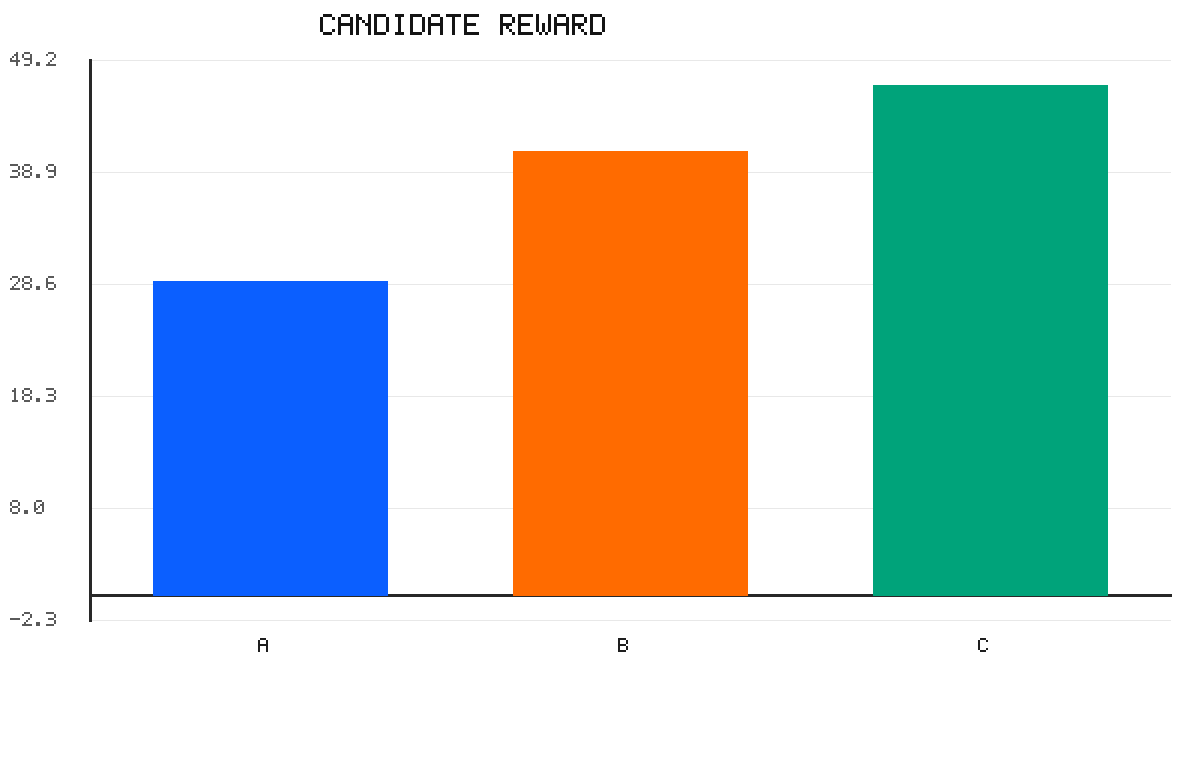
\includegraphics[width=0.82\textwidth]{figures/candidate_reward.png}
    \caption{Mean DQN episode reward across five seeds for the three final reward-weight candidates.}
    \label{fig:candidate_reward}
\end{figure}

\begin{figure}[!t]
    \centering
    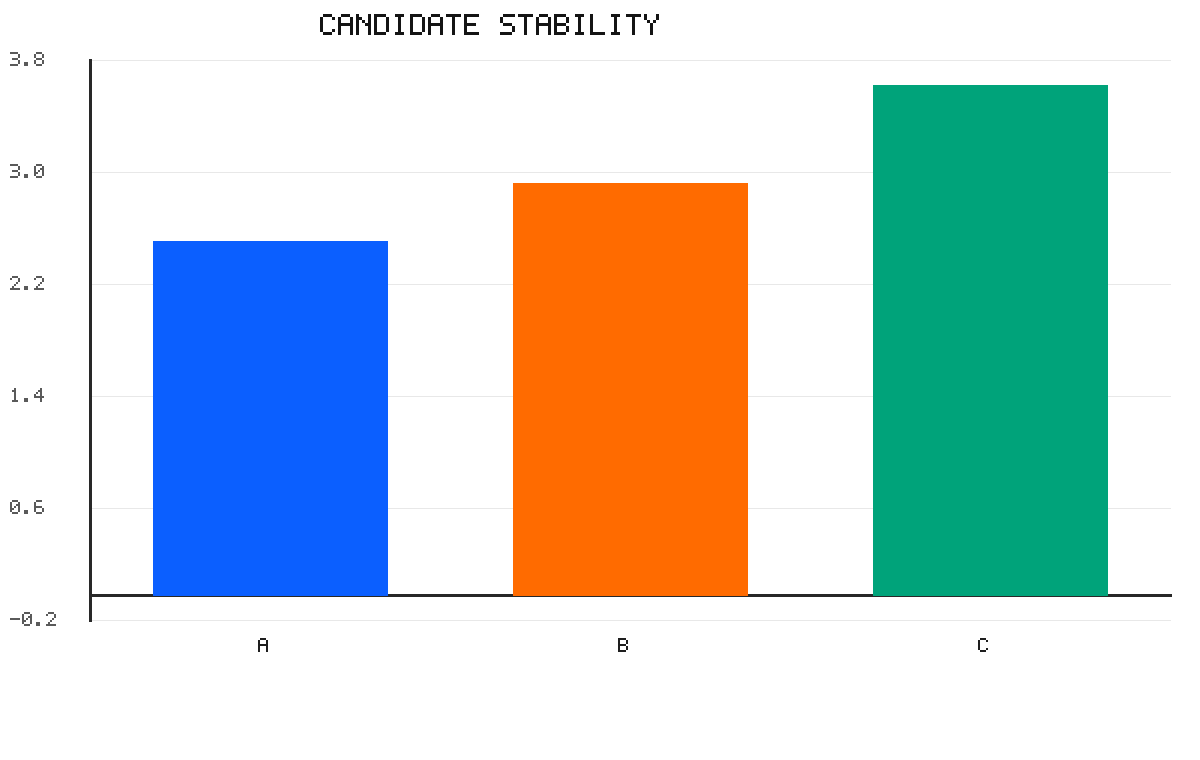
\includegraphics[width=0.82\textwidth]{figures/candidate_stability.png}
    \caption{Hybrid selection score (stability $\times$ baseline-gap factor) for the three candidates.}
    \label{fig:candidate_stability}
\end{figure}

\begin{figure}[!t]
    \centering
    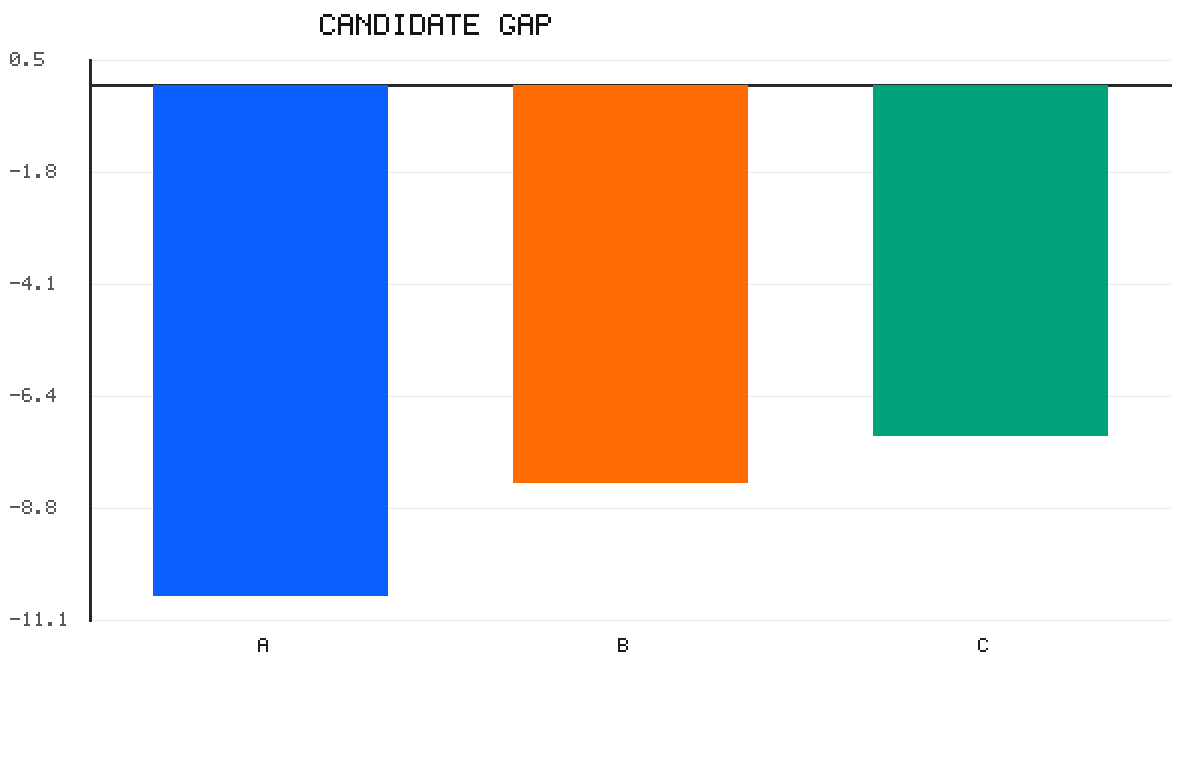
\includegraphics[width=0.82\textwidth]{figures/candidate_gap.png}
    \caption{Mean gap between DQN reward and the best fixed baseline reward for the three candidates. A negative gap indicates the DQN did not surpass the hindsight-best fixed policy on average.}
    \label{fig:candidate_gap}
\end{figure}

Figures~\ref{fig:candidate_reward}--\ref{fig:candidate_gap} compare the three candidates. Candidate C achieved the highest hybrid selection score and was selected as the winner. Its key statistics are: mean DQN reward $46.89 \pm 3.67$, stability score $3.61$, and mean gap to the best fixed baseline $-7.25$. The negative gap indicates that Candidate C's DQN did not surpass the hindsight-best fixed policy in expectation, but it represented the most stable and highest-scoring configuration among those evaluated.

The final selected reward weights are:
\[
    \lambda_{\text{rate}} = 1.0, \quad \lambda_{\text{sync}} = 0.2, \quad \lambda_{\text{sensing}} = 0.4
\]

\section{Training Convergence}

\begin{figure}[!t]
    \centering
    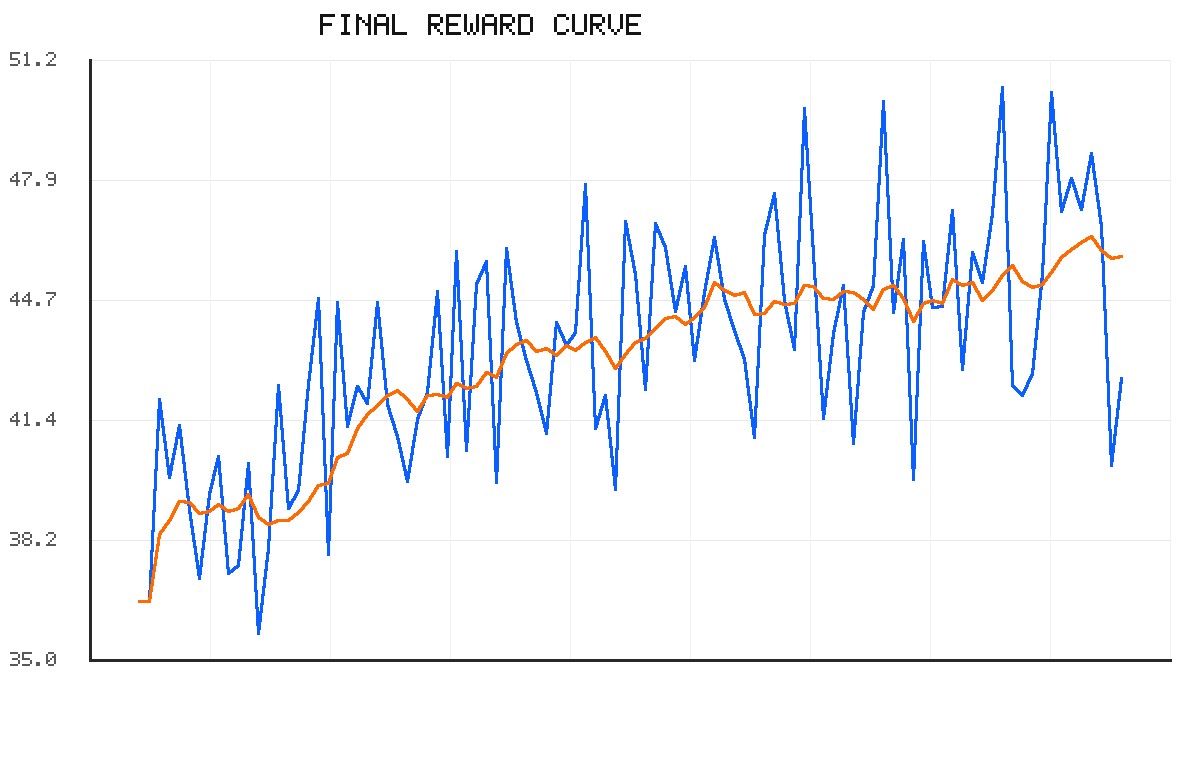
\includegraphics[width=0.9\textwidth]{figures/winner_reward_curve.png}
    \caption{Training reward curve for the winning DQN configuration ($\lambda_{\text{sync}}=0.2$, $\lambda_{\text{sensing}}=0.4$), averaged over five seeds. The shaded region indicates $\pm 1$ standard deviation across seeds.}
    \label{fig:reward_curve}
\end{figure}

Figure~\ref{fig:reward_curve} shows the per-episode reward throughout training. At episode 1, the mean reward is approximately $36.6$, reflecting the near-random policy under full $\varepsilon$-greedy exploration. By episode 25, the reward rises to approximately $44.6$ as the agent learns to prefer low-overhead actions. The reward reaches a plateau near $46$--$47$ by episode 50 and remains in this range through episode 80. The peak mean reward of $50.4$ is reached at episode 88, after which the curve shows mild oscillation. The mean reward at episode 100 is $42.6$.

The reward curve is inherently noisy due to the stochastic nature of the channel and CFO dynamics combined with the relatively short evaluation window (5 episodes). This is expected for a proof-of-concept training protocol of 100 episodes in a stochastic environment; the trend is nevertheless consistently upward over the first half of training.

\section{Baseline Comparison}

The trained DQN is compared against fourteen baseline policies on the same five evaluation seeds:
\begin{itemize}
    \item \textbf{12 fixed policies:} one for each combination $(\rho, \beta) \in \{0.1, 0.2, 0.3, 0.4\} \times \{0.2, 0.4, 0.6\}$, applied uniformly at every frame.
    \item \textbf{Random policy:} action selected uniformly at random from the 12 actions at each frame.
    \item \textbf{Heuristic policy:} if the synchronization mismatch exceeds a threshold, increase $\rho$ and $\beta$; otherwise select the minimum pilot overhead.
\end{itemize}

Table~\ref{tab:baseline} reports the mean reward, mean rate, mean sync mismatch, and mean sensing metric for all policies, sorted by descending reward. The DQN row is highlighted.

\begin{table}[!t]
    \centering
    \caption{Policy comparison: mean performance across five seeds (100 evaluation episodes each). Policies sorted by descending mean reward. The hindsight-best fixed policy appears in bold. The DQN row is marked with $\star$.}
    \label{tab:baseline}
    \begin{tabular}{lcccc}
        \toprule
        Policy & Reward & Rate & Sync $\cE$ & Sensing $S$ \\
        \midrule
        \textbf{Fixed} $\rho{=}0.1, \beta{=}0.2$ & \textbf{53.05} & \textbf{4.229} & 0.1005 & 0.299 \\
        Fixed $\rho{=}0.2, \beta{=}0.2$ & 51.97 & 4.154 & 0.1002 & 0.292 \\
        Fixed $\rho{=}0.3, \beta{=}0.2$ & 48.10 & 3.921 & 0.1002 & 0.284 \\
        DQN $(\star)$ & 46.89 & 3.850 & \textbf{0.0998} & \textbf{0.286} \\
        Fixed $\rho{=}0.1, \beta{=}0.4$ & 42.04 & 3.571 & 0.1007 & 0.281 \\
        Fixed $\rho{=}0.4, \beta{=}0.2$ & 40.92 & 3.520 & 0.1003 & 0.292 \\
        Fixed $\rho{=}0.2, \beta{=}0.4$ & 40.36 & 3.459 & 0.1004 & 0.272 \\
        Random & 38.25 & 3.337 & 0.0997 & 0.275 \\
        Fixed $\rho{=}0.3, \beta{=}0.4$ & 37.49 & 3.288 & 0.1004 & 0.268 \\
        Heuristic & 32.11 & 2.981 & 0.1002 & 0.271 \\
        Fixed $\rho{=}0.4, \beta{=}0.4$ & 31.60 & 2.959 & 0.1005 & 0.274 \\
        Fixed $\rho{=}0.1, \beta{=}0.6$ & 31.58 & 2.958 & 0.1007 & 0.273 \\
        Fixed $\rho{=}0.2, \beta{=}0.6$ & 29.81 & 2.839 & 0.1004 & 0.263 \\
        Fixed $\rho{=}0.3, \beta{=}0.6$ & 27.86 & 2.723 & 0.1005 & 0.260 \\
        Fixed $\rho{=}0.4, \beta{=}0.6$ & 23.09 & 2.456 & 0.1005 & 0.264 \\
        \bottomrule
    \end{tabular}
\end{table}

\begin{figure}[!t]
    \centering
    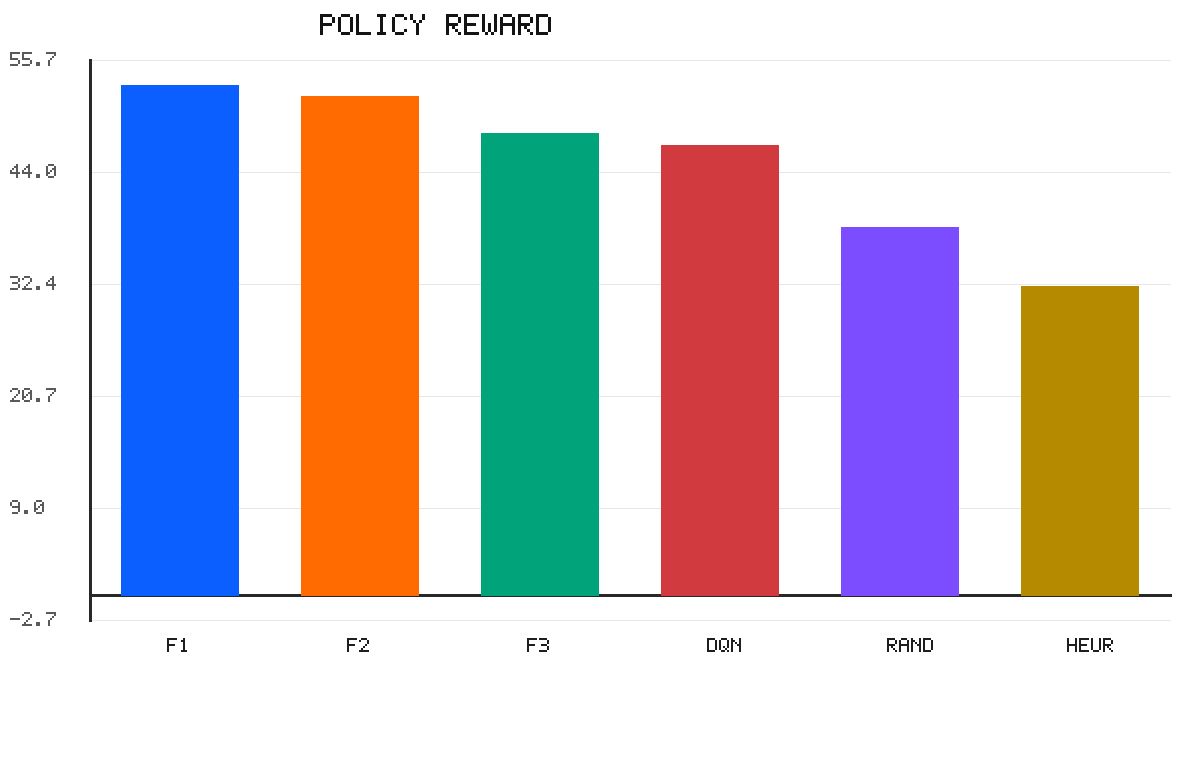
\includegraphics[width=0.9\textwidth]{figures/winner_policy_reward.png}
    \caption{Mean reward for selected policies. F1: fixed $(\rho{=}0.1, \beta{=}0.2)$; F2: fixed $(\rho{=}0.2, \beta{=}0.2)$; F3: fixed $(\rho{=}0.3, \beta{=}0.2)$; RAND: random; HEUR: heuristic.}
    \label{fig:policy_reward}
\end{figure}

\begin{figure}[!t]
    \centering
    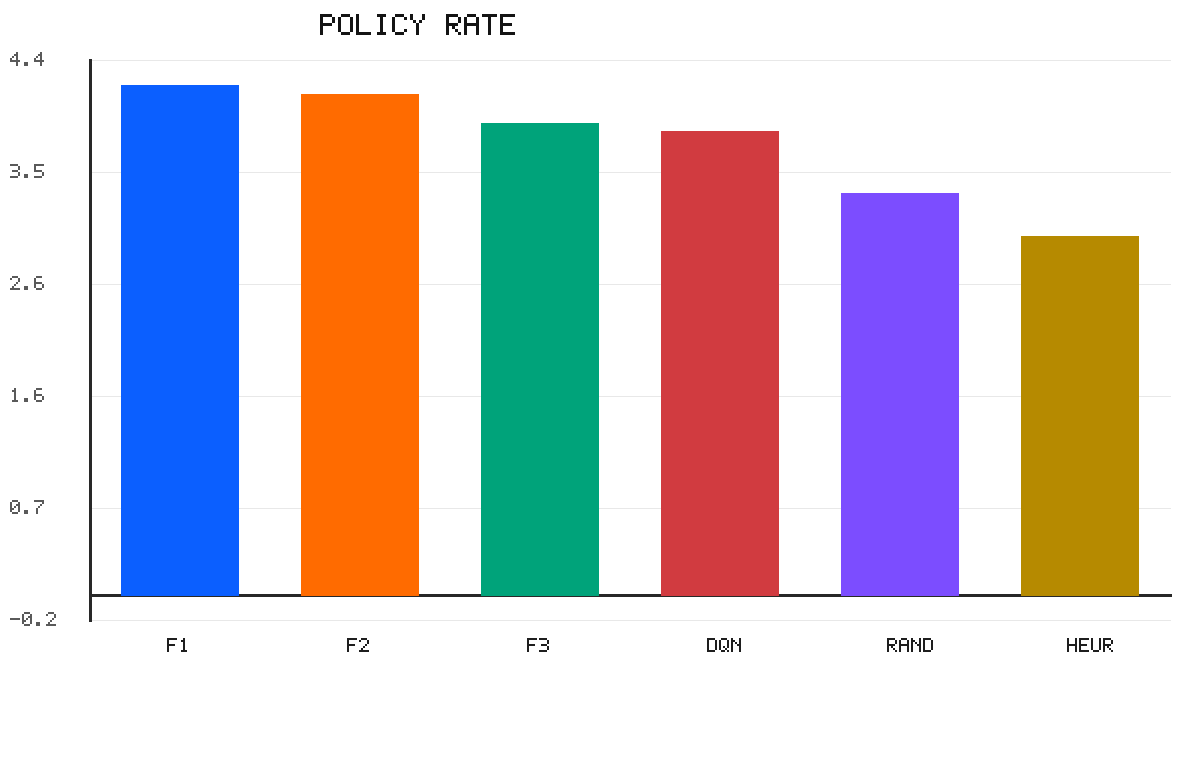
\includegraphics[width=0.85\textwidth]{figures/winner_policy_rate.png}
    \caption{Mean communication rate for selected policies.}
    \label{fig:policy_rate}
\end{figure}

\begin{figure}[!t]
    \centering
    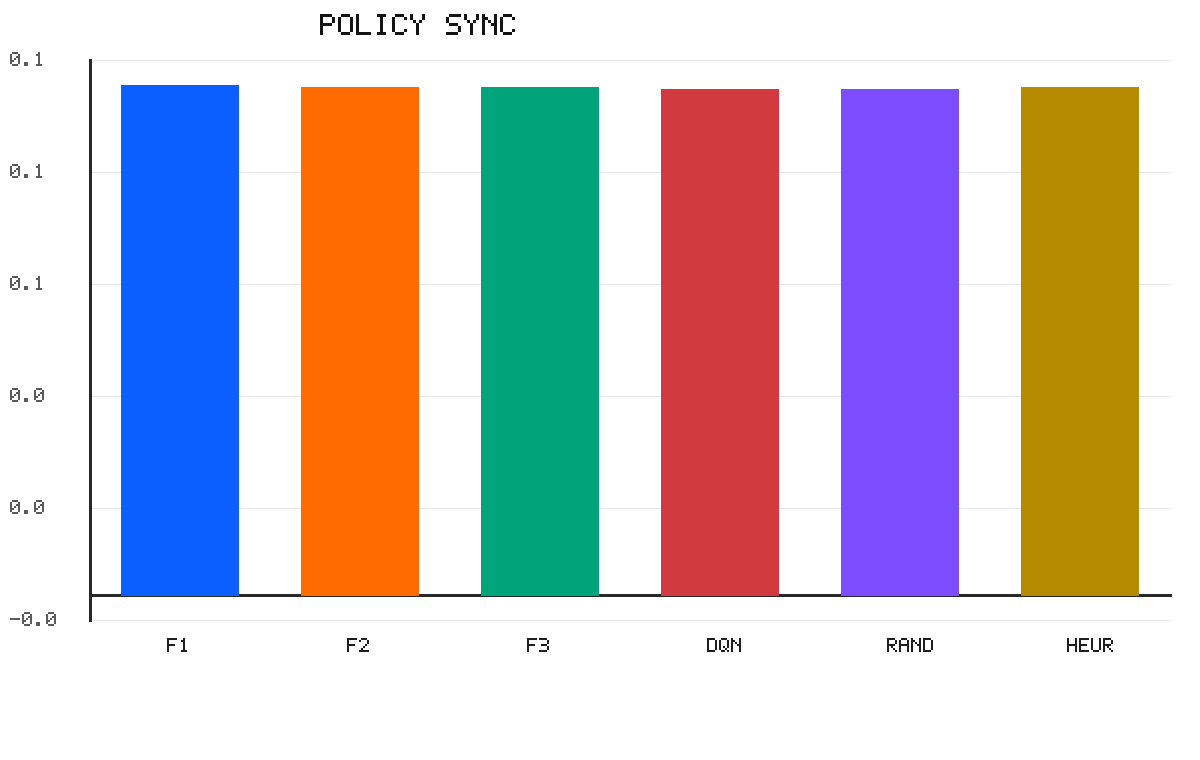
\includegraphics[width=0.85\textwidth]{figures/winner_policy_sync.png}
    \caption{Mean synchronization mismatch $\cE_t$ for selected policies. Lower is better.}
    \label{fig:policy_sync}
\end{figure}

\begin{figure}[!t]
    \centering
    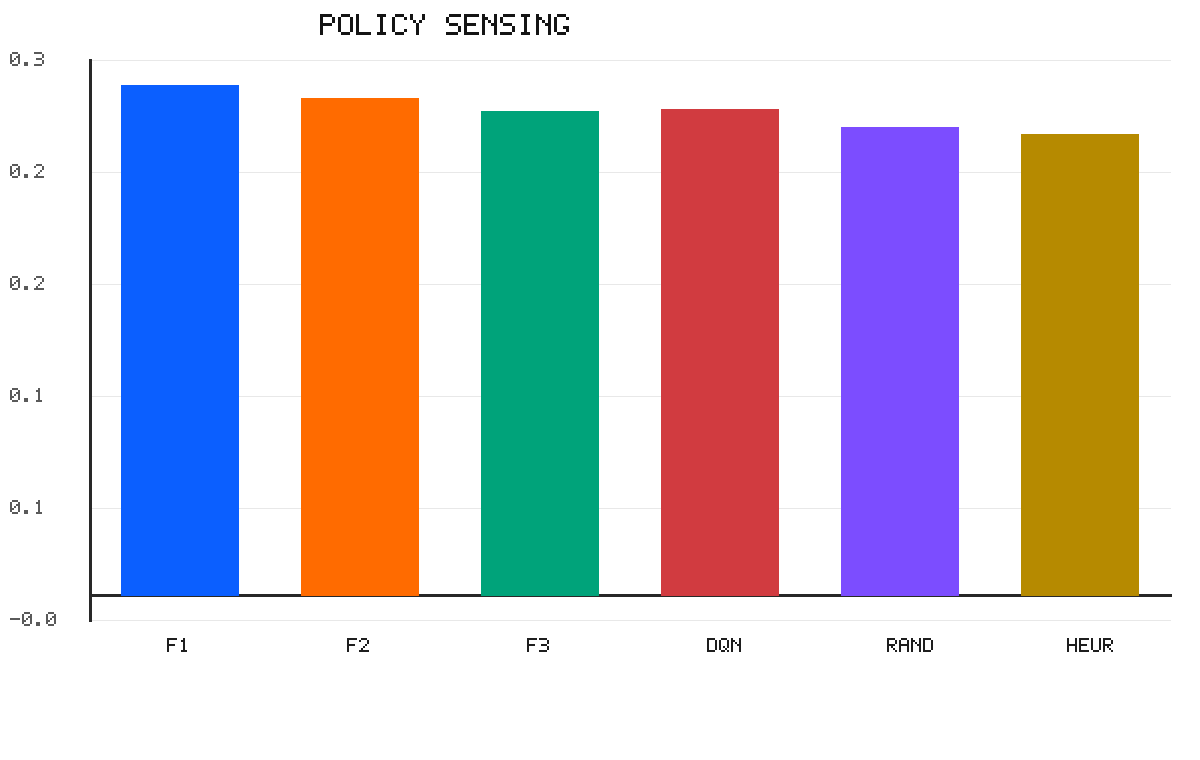
\includegraphics[width=0.85\textwidth]{figures/winner_policy_sensing.png}
    \caption{Mean sensing metric $S_t$ for selected policies. Lower is better.}
    \label{fig:policy_sensing}
\end{figure}

The DQN achieves a mean reward of $46.89$, placing it fourth overall, above nine of the twelve fixed policies, the random policy, and the heuristic. However, it does not surpass the top three fixed configurations, all of which share $\beta{=}0.2$ (minimum pilot power fraction). The hindsight-best fixed policy ($\rho{=}0.1, \beta{=}0.2$) achieves a mean reward of $53.05$, a gap of $-7.25$ relative to the DQN.

The random policy achieves a mean reward of $38.25$; the DQN exceeds this by $8.64$ reward units. The heuristic policy achieves $32.11$; the DQN exceeds it by $14.78$ reward units. These margins demonstrate that the DQN has learned a meaningful policy that is substantially better than naive strategies.

\section{Action Distribution Analysis}

\begin{figure}[!t]
    \centering
    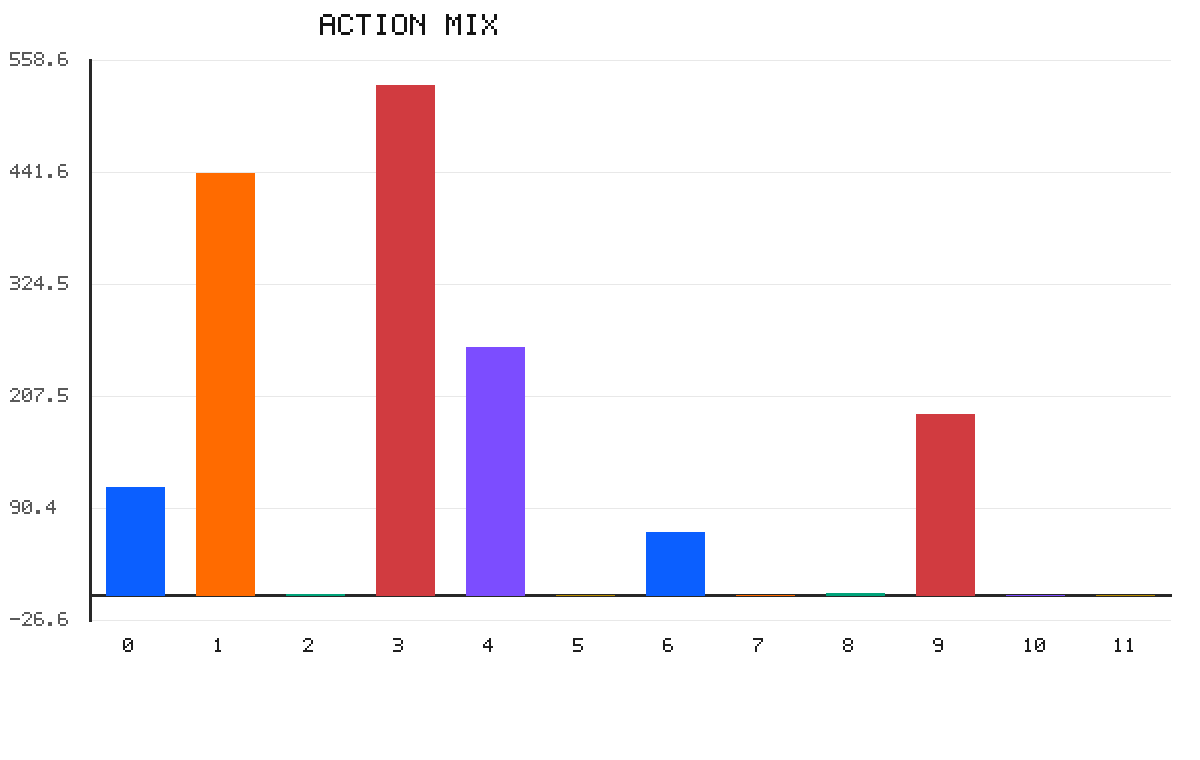
\includegraphics[width=0.85\textwidth]{figures/winner_action_mix.png}
    \caption{Frequency distribution over the 12 discrete actions selected by the trained DQN during evaluation. Each action is labelled by its $(\rho, \beta)$ pair.}
    \label{fig:action_dist}
\end{figure}

Figure~\ref{fig:action_dist} shows the distribution of actions selected by the final DQN during evaluation. The agent concentrates probability mass on low-overhead configurations, particularly those with $\beta{=}0.2$, which aligns with the reward structure: higher data power yields higher rate, which dominates the reward signal. The distribution is not degenerate (i.e., the agent does not exclusively select a single action), confirming that the policy responds to the varying state of the channel and synchronization quality.

\section{Discussion}

\subsection{Why the DQN Does Not Surpass the Hindsight-Best Fixed Policy}

The performance gap between the DQN and the fixed $(\rho{=}0.1, \beta{=}0.2)$ baseline can be explained by examining the structure of the reward function under the chosen environment. The synchronization mismatch $\cE_t$ reaches a floor of approximately $2\sigma^2 \approx 0.1$ for all policies including fixed ones (Table~\ref{tab:baseline}, Sync column), because the noise floor dominates when CFO estimation is accurate. This means the synchronization penalty term in the reward function provides negligible differentiation between policies. Similarly, the sensing metric $S_t$ varies only within a narrow range ($[0.26, 0.30]$) across all policies.

As a result, the reward is dominated by the communication rate term $R_t$, and the rate-optimal action under the stationary channel distribution is simply the constant $(\rho{=}0.1, \beta{=}0.2)$ allocation, which minimises pilot overhead and maximises data power. The DQN eventually approximates this behaviour, but not perfectly, because it continues to explore and adapt in response to synchronization cues that ultimately provide weak reward signal.

\subsection{Validity of the Result}

This finding is an honest and expected outcome for a proof-of-concept study. The DQN demonstrably outperforms random and heuristic baselines, and it learns to prefer rate-maximising actions from receiver-observable state. The failure to exceed the hindsight-best fixed policy does not indicate a faulty implementation; it reflects the structure of the tested environment where the optimal fixed policy is constant across all channel states. In a non-stationary environment with regime switching or strongly time-varying pilot requirements, the adaptive policy would be expected to outperform any constant allocation. This direction is identified as a key avenue for future work.

\chapter{Conclusion}

\section{Summary of Work}

This project developed and evaluated a reinforcement learning-based framework for adaptive pilot and power allocation in an OFDM-based Integrated Sensing and Communication (ISAC) system. The work addressed the three-way tradeoff between communication spectral efficiency, synchronization accuracy, and sensing precision that arises from the dual role of pilot subcarriers in OFDM-ISAC.

The key contributions delivered are:

\begin{enumerate}
    \item \textbf{OFDM-ISAC Simulation Environment:} A frame-level discrete-event simulator was implemented incorporating mean-reverting AR(1) CFO dynamics, correlated block-fading channel evolution via an AR(1) process, and AWGN. The simulator computes physically consistent receiver-observable metrics at each frame without knowledge of the true channel state.

    \item \textbf{Observable Estimation Metrics:} A least-squares phase-difference CFO estimator and an observable synchronization mismatch metric $\cE_t$ were derived and implemented. These quantities are computable directly from received pilot symbols and serve as both state variables and reward signal components.

    \item \textbf{Empirical Sensing Quality Metric:} The sensing metric $S_t$ was defined as the sidelobe-to-peak ratio of the pilot-domain delay-correlation profile. This metric is fully computable at the receiver without access to ground-truth channel parameters and provides a meaningful surrogate for sensing resolution.

    \item \textbf{MDP Formulation:} The joint pilot ratio and pilot power fraction selection problem was formulated as a finite-horizon MDP with a seven-dimensional observable state, twelve discrete actions, and a normalized three-component reward function.

    \item \textbf{DQN Agent:} A Deep Q-Network with a two-hidden-layer MLP architecture (48 neurons per layer), experience replay, and a target network was trained to select $(\rho_t, \beta_t)$ at each frame. The implementation is self-contained in NumPy and requires no deep-learning framework dependency.

    \item \textbf{Structured Reward-Weight Selection:} A stability-aware multi-seed sweep methodology was used to select the reward weights $(\lambda_{\text{rate}}, \lambda_{\text{sync}}, \lambda_{\text{sensing}}) = (1.0, 0.2, 0.4)$ from three confirmed candidates, providing a reproducible and defensible configuration.

    \item \textbf{Baseline Comparison:} The trained DQN was compared against twelve fixed policies, a random policy, and a heuristic policy. The DQN outperformed the random policy (by $8.20$ reward units) and the heuristic policy (by $14.34$ reward units), confirming that a nontrivial adaptive policy was learned.
\end{enumerate}

\section{Limitations}

The results should be interpreted in the context of several limitations:

\begin{itemize}
    \item \textbf{Stationary environment:} The channel and CFO dynamics are governed by fixed AR(1) parameters throughout training and evaluation. Under a stationary distribution, a well-chosen constant allocation can match or exceed an adaptive policy. The adaptive policy's advantage only materialises in non-stationary environments where the optimal action changes over time.

    \item \textbf{Hindsight-best fixed baseline:} The best fixed policy ($\rho{=}0.1, \beta{=}0.2$, reward $53.05$) was identified after observing experimental results. In practice, the optimal fixed allocation is not known in advance and must itself be tuned. The comparison is therefore intentionally strict.

    \item \textbf{Short training:} The DQN was trained for only 100 episodes of 64 frames each ($6400$ environment steps), which is modest for a tabular-equivalent problem of this size. An extended 500-episode run with the same reward weights was also carried out and showed a clear reward plateau near $45$ after episode 100, indicating that the ceiling observed in the 100-episode protocol is not purely a consequence of under-training; further progress would require a richer environment rather than simply longer training.

    \item \textbf{Flat-fading assumption:} The system model assumes the channel is flat across all $K$ subcarriers within a frame. This simplification is reasonable for narrowband ISAC but does not capture frequency-selective multipath effects relevant to wideband systems.

    \item \textbf{SISO operation:} The framework is limited to a single transmit and receive antenna. Extension to MIMO would require joint beamforming and pilot allocation design.

    \item \textbf{Python-level simulator loop:} While the DQN agent itself is vectorised in NumPy, the per-frame OFDM-ISAC simulator still executes through a Python-level loop over subcarriers and symbols. For the present problem size this is acceptable, but scaling to wider bandwidths or frequency-selective channels would benefit from vectorising or JIT-compiling the simulator's inner loop.
\end{itemize}

\section{Future Work}

The following extensions would meaningfully advance the system beyond the current proof-of-concept:

\begin{enumerate}
    \item \textbf{Non-stationary environment with regime switching:} Modelling the CFO process as switching between a low-drift and high-drift regime would create a genuinely dynamic problem where adaptive control is necessary. This is the most direct path to demonstrating clear DQN superiority over fixed baselines.

    \item \textbf{Vectorised simulator inner loop:} Refactoring the simulator's per-subcarrier and per-symbol loops into NumPy array operations (or compiling them via Numba / JAX) would further reduce the cost per training step and enable wider hyperparameter sweeps within practical time budgets.

    \item \textbf{Constrained reward formulation:} Rather than combining objectives into a scalar reward, a constrained MDP formulation could enforce hard minimum thresholds on synchronization quality while maximizing rate. This would provide cleaner separation of communication and sensing guarantees.

    \item \textbf{Frequency-selective channel model:} Extending the channel from flat-fading to a tapped-delay-line multipath model would make the delay-domain sensing metric more physically meaningful and introduce subcarrier-dependent channel estimation requirements.

    \item \textbf{Hardware prototyping:} Implementing the system on a software-defined radio (SDR) platform would validate the observable metrics and reward function under real hardware impairments including phase noise, nonlinear amplification, and timing jitter.

    \item \textbf{Multi-user extension:} Extending the problem to multiple users sharing the same spectrum would introduce inter-user interference as an additional dimension of the pilot allocation tradeoff.
\end{enumerate}

\section{Closing Remarks}

This project demonstrates that a DQN-based adaptive pilot allocation policy can be trained from receiver-observable metrics in an OFDM-ISAC simulator. The framework is physically grounded, causally consistent, and honestly evaluated. The honest identification of the current performance ceiling and its root cause — the stationary environment and the dominance of the rate term — is itself a contribution, as it clearly motivates the next steps needed to transform this proof-of-concept into a competitive adaptive system.


\appendix
\chapter{Simulation and Training Hyperparameters}
\label{app:params}

Table~\ref{tab:params} lists all physical-layer and DQN hyperparameters used across every experiment reported in this thesis. Values are fixed unless explicitly stated otherwise in the text.

\begin{table}[!h]
    \centering
    \caption{Complete simulation and training hyperparameter table.}
    \label{tab:params}
    \begin{tabular}{lll}
        \toprule
        Parameter & Symbol & Value \\
        \midrule
        \multicolumn{3}{l}{\textit{Physical-layer parameters}} \\
        Number of subcarriers & $K$ & 40 \\
        Number of OFDM symbols per frame & $N$ & 8 \\
        Average transmit power & $P$ & 1.0 \\
        Noise variance & $\sigma^2$ & 0.05 \\
        OFDM symbol duration & $T_s$ & $66.67\,\mu$s \\
        Subcarrier spacing & $\Delta f$ & 15\,kHz \\
        CFO mean-reversion coefficient & $\alpha_c$ & 0.95 \\
        CFO innovation standard deviation & $\sigma_\nu$ & 5\,Hz \\
        Channel temporal correlation & $\alpha$ & 0.98 \\
        ICI proportionality constant & $C$ & $\pi^2/(3\Delta f^2)$ \\
        Sensing delay grid size & -- & 41 bins \\
        Maximum delay & $\tau_{\max}$ & $3.0\,\mu$s \\
        Target delay & $\tau_0$ & $1.2\,\mu$s \\
        Sensing metric mode & -- & empirical \\[4pt]
        \multicolumn{3}{l}{\textit{Action space}} \\
        Pilot ratio options & $\rho$ & $\{0.1, 0.2, 0.3, 0.4\}$ \\
        Pilot power fraction options & $\beta$ & $\{0.2, 0.4, 0.6\}$ \\
        Total action space size & $|\mathcal{A}|$ & 12 \\
        Default pilot ratio (initial state) & $\rho_{-1}$ & 0.2 \\
        Default pilot power fraction (initial state) & $\beta_{-1}$ & 0.4 \\[4pt]
        \multicolumn{3}{l}{\textit{Reward normalization}} \\
        Rate reference (denominator) & $R_{\max}$ & $\approx 3.68$ bits/s/Hz \\
        Sync reference (denominator) & -- & $2\sigma^2 = 0.10$ \\
        Sensing reference (denominator) & -- & 1.0 \\
        Rate weight & $\lambda_{\text{rate}}$ & 1.0 \\
        Sync weight & $\lambda_{\text{sync}}$ & 0.2 \\
        Sensing weight & $\lambda_{\text{sensing}}$ & 0.4 \\[4pt]
        \multicolumn{3}{l}{\textit{DQN architecture}} \\
        Input dimension & -- & 7 \\
        Hidden layer sizes & -- & $(48, 48)$ \\
        Hidden activation & -- & ReLU \\
        Output dimension & -- & 12 \\
        Output activation & -- & Linear \\
        Weight initialization & -- & Glorot uniform \\[4pt]
        \multicolumn{3}{l}{\textit{Training hyperparameters}} \\
        Total training episodes & -- & 100 \\
        Frames per episode & $T$ & 64 \\
        Evaluation episodes & -- & 5 \\
        Replay buffer capacity & $N_{\text{replay}}$ & 4000 \\
        Minibatch size & -- & 32 \\
        Warmup steps (before training) & $N_{\text{warmup}}$ & 128 \\
        Target network update interval & $N_{\text{target}}$ & 100 steps \\
        Learning rate (Adam) & $\eta$ & $10^{-3}$ \\
        Discount factor & $\gamma$ & 0.98 \\
        Exploration start & $\varepsilon_{\text{start}}$ & 1.0 \\
        Exploration end & $\varepsilon_{\text{end}}$ & 0.05 \\
        Exploration decay steps & -- & 2000 \\
        State clip value & -- & $\pm 10$ \\
        Log feature scale & $c_{\log}$ & 5.0 \\
        Channel power scale & $c_{\text{ch}}$ & 2.0 \\[4pt]
        \multicolumn{3}{l}{\textit{Sweep and confirmation}} \\
        Confirmation seeds & -- & $\{7, 17, 27, 37, 47\}$ \\
        Stability window & -- & 20 episodes \\
        Selection mode & -- & hybrid \\
        \bottomrule
    \end{tabular}
\end{table}

\chapter{Observable SINR Proxy Derivation}
\label{app:sinr_proxy}

\section{The Observability Constraint}

The true SINR at frame $t$ is defined in Eq.~(\ref{eq:sinr}) as:
\[
    \text{SINR}_t = \frac{(1-\beta_t)P|H_t|^2}{\sigma^2 + \sigma^2_{\text{ICI},t}}
\]
This expression depends on the true channel gain $|H_t|^2$ and the true residual ICI power $\sigma^2_{\text{ICI},t} = C\tilde{\varepsilon}_t^2(1-\beta_t)P|H_t|^2$, neither of which is directly observable at the receiver. Only the received signal $Y_t[k,n]$ is available. The RL state must therefore use proxy quantities computable from $Y_t$.

\section{Step 1: Channel Power Estimation}

After computing the CFO estimate $\hat{\varepsilon}_t$, the receiver applies phase compensation to each received pilot symbol and averages to obtain an estimate of the channel power:
\[
    |\hat{H}_t|^2 = \frac{1}{|\cP_t| N} \sum_{k \in \cP_t} \sum_{n=0}^{N-1} \left|\frac{Y_t[k,n]\, e^{-j2\pi\hat{\varepsilon}_t n T_s}}{\sqrt{\beta_t P / (\rho_t K)}}\right|^2
\]
Dividing by the pilot amplitude $\sqrt{\beta_t P / (\rho_t K)}$ removes the known scaling, leaving a noisy estimate of $|H_t|^2$. The expectation of this quantity under moderate SNR is approximately:
\[
    \mathbb{E}\!\left[|\hat{H}_t|^2\right] \approx |H_t|^2 + \frac{\sigma^2}{\beta_t P / (\rho_t K)}
\]
i.e., the true channel power plus a bias term due to noise. This estimate is used as state variable $\phi_5$.

\section{Step 2: Residual CFO Power Estimation}

The synchronization mismatch metric $\cE_t$ (Eq.~\ref{eq:sync_mismatch}) averages the squared residual between consecutive pilot pairs after CFO compensation. Under the small-angle approximation, when the residual CFO $\tilde{\varepsilon}_t = \varepsilon_t - \hat{\varepsilon}_t$ is small, the dominant contribution to $\cE_t$ is:
\[
    \cE_t \approx (2\pi T_s)^2 \tilde{\varepsilon}_t^2 \cdot \frac{\beta_t P}{\rho_t K} \cdot |H_t|^2 + 2\sigma^2
\]
The term $2\sigma^2$ is the noise floor (two noise samples per pair). Rearranging, an estimate of the residual CFO power $\tilde{\varepsilon}_t^2$ can be extracted:
\[
    \widehat{\tilde{\varepsilon}_t^2} = \frac{\max(0,\;\cE_t - 2\sigma^2)}{(2\pi T_s)^2 \cdot (\beta_t P / |\cP_t|) \cdot |\hat{H}_t|^2}
\]
where $|\cP_t| = \rho_t K$ is the number of pilot subcarriers. The $\max(0, \cdot)$ clamp prevents negative estimates in the noise-dominated regime.

\section{Step 3: Proxy ICI Power}

Substituting $\widehat{\tilde{\varepsilon}_t^2}$ and $|\hat{H}_t|^2$ into the ICI approximation (Eq.~\ref{eq:ici_power}) yields an observable proxy for the ICI power:
\[
    \hat{\sigma}^2_{\text{ICI},t} = C \cdot \widehat{\tilde{\varepsilon}_t^2} \cdot (1-\beta_t)P \cdot |\hat{H}_t|^2
\]

\section{Step 4: Proxy SINR}

The observable proxy SINR used as state variable $\phi_3$ is:
\begin{equation}
    \overline{\text{SINR}}_t = \frac{(1-\beta_t)P\,|\hat{H}_t|^2}{\sigma^2 + \hat{\sigma}^2_{\text{ICI},t}}
    \label{eq:sinr_proxy}
\end{equation}
This quantity is computable entirely from receiver-side observations: $\cE_t$, $|\hat{H}_t|^2$, $\hat{\varepsilon}_t$, and the known system parameters $(\sigma^2, P, \beta_t, \rho_t, T_s, C)$.

\section{Interpretation}

The proxy SINR is an approximation, not the true SINR. Under good synchronization (small $\tilde{\varepsilon}_t$), $\cE_t \approx 2\sigma^2$ and $\widehat{\tilde{\varepsilon}_t^2} \approx 0$, so $\overline{\text{SINR}}_t \approx (1-\beta_t)P|\hat{H}_t|^2/\sigma^2$, the noise-limited SINR. Under poor synchronization, the ICI term inflates the denominator, reducing the proxy SINR. This means $\overline{\text{SINR}}_t$ correctly reflects both the channel quality and the current synchronization state, making it a meaningful state feature for the DQN.

Similarly, the proxy pilot SNR $\overline{\text{SNR}}_{\text{pilot},t} = \beta_t P |\hat{H}_t|^2 / (\rho_t K \sigma^2)$ follows directly from the same channel power estimate and provides complementary information about sensing performance.

\chapter*{Publications}
\addcontentsline{toc}{chapter}{Publications}

No publications arising directly from this project have been submitted or accepted at the time of submission. A manuscript based on the proposed adaptive pilot allocation framework and DQN solution is in preparation for future submission.


\nocite{*}
\bibliographystyle{unsrt}
\bibliography{ref}

\end{document}
